\chapter{Clustering}
Le tecniche di apprendimento si possono dividere in:
\begin{itemize}
      \item \textbf{Supervisionato}: ad ogni istanza del dataset è associata una
            label che indica la classe di appartenenza.
      \item \textbf{Non supervisionato}: le istanze del dataset non son etichettate,
            si cerca di trovare una regola che spieghi il dataset.
\end{itemize}
Spesso si può usare l'apprendimento non supervisionato al posto del supervisionato,
perché potrebbe ottenere dei risultati migliori, soprattutto quando il dataset è
pieno di rumore. I sistemi non supervisionati tornano comodi quando la distribuzione
dei valori degli attributi è informazione sufficiente per separare le istanze in
più classi, si hanno quindi domini dove questo fattore è determinante.

Il fatto di utilizzare un apprendimento non supervisionato porta a diversi
\textbf{vantaggi}:
\begin{itemize}
      \item Non è richiesta alcuna conoscenza a priori quindi evito problemi legati
            ad eventuali etichette errate (errori umani ridotti).
      \item Tutte le classi che hanno caratteristiche uniche vengono identificate.
      \item Efficaci con elementi di tipo numerico perché vengono rappresentate in
            uno spazio di punti o di ordinamento intrinseco grazie al calcolo delle
            distanze.
\end{itemize}
I \textbf{lati negativi} dell'apprendimento non supervisionato sono:
\begin{itemize}
      \item Le classi ottenute potrebbero non avere significati.
      \item L'utente ha poco controllo sulla procedura e sui risultati.
      \item Scarsa efficacia su elementi ordinati in modo arbitrario o parziale.
\end{itemize}
Il \textbf{clustering} consiste nel  separare, categorizzare, raggruppare in
autonomia con un apprendimento \textbf{non supervisionato}.
Per il clustering, la fase di apprendimento cambia, ma la fase predizione rimane
identica perché ho trovato una regola che spiega il dataset. Il criterio per cui
raggruppare è arbitrario, non si conoscono il numero di gruppi in cui partizionare
il dataset e si dovrà trovare un modo per valutare il raggruppamento ottenuto.

In sostanza si cerca una regola che possa spiegare come raggruppare i dati senza
avere una label di riferimento e il numero di gruppi. La ricerca del raggruppamento
migliore si baserà sempre sulla ricerca dell'ipotesi più semplice. Non conoscendo
le label allora raggrupperemo sfruttando le \textbf{distanze}, ovvero un elemento
fa parte di un raggruppamento noto se si trova vicino agli elementi di quel
raggruppamento.

I dati che vengono utilizzati per effettuare il clustering sono principalmente
vettori numerici, dove ogni elemento misura una specifica \textbf{caratteristica}
(\textbf{feature}) dell'istanza. Per poter raggruppare questi elementi è necessario
definire dei criteri di similarità tra i vettori.

Si hanno quindi due criteri da rispettare:
\begin{itemize}
      \item \textbf{Omogeneità}: gli elementi di un cluster devono essere simili
            tra loro.
      \item \textbf{Separazione}: gli elementi di cluster diversi devono essere
            dissimili tra loro.
\end{itemize}
\begin{definizione}[\textbf{Cluster}]
      Sia $N = \{e_1, \dots, e_n\}$ l'insieme degli elementi da raggruppare e sia
      $C = \{c_1, \dots, c_k\}$ una partizione di $N$ in sottoinsiemi disgiunti
      $C_i$. Ogni sottoinsieme $C_i$ è un \textbf{cluster}. Due elementi si
      chiamano \textbf{mates} rispetto a $C$ se sono membri dello stesso cluster.
\end{definizione}
\begin{definizione}[\textbf{Misura di similarità}]
      Possiamo definire una \textbf{misura di similarità} tra due elementi $e_i$ e
      $e_j$ utilizzando la distanza. In particolare possiamo utilizzare:
      \begin{itemize}
            \item \textbf{Distanza euclidea}: invariante rispetto a traslazioni
                  e rotazioni degli assi, rappresenta la lunghezza del segmento
                  tra i due punti.
                  \begin{equation}
                        d(e_i, e_j) = \sqrt{\sum_{k=1}^n (e_{ik} - e_{jk})^2}
                  \end{equation}
            \item \textbf{Distanza di Manhattan}: non è invariante rispetto a
                  traslazioni o rotazioni degli assi.
                  \begin{equation}
                        d(e_i, e_j) = \sum_{k=1}^n |e_{ik} - e_{jk}|
                  \end{equation}
            \item \textbf{Distanza di Minkowski}:
                  \begin{equation}
                        d(e_i, e_j) = \sqrt[p]{\sum_{k=1}^n |e_{ik} - e_{jk}|^p}
                  \end{equation}
                  \begin{itemize}
                        \item La distanza di Manhattan è un caso particolare
                              della distanza di Minkowski con $p = 1$.
                        \item La distanza euclidea è un caso particolare della
                              distanza di Minkowski con $p = 2$.
                        \item La distanza di Chebyshev è un caso particolare
                              della distanza di Minkowski con $p = \infty$.
                  \end{itemize}
      \end{itemize}
\end{definizione}
Esistono diversi tipi di clustering, possiamo principalmente individuare:
\begin{itemize}
      \item \textbf{Clustering gerarchico}: si costruisce una gerarchia di cluster.
            Si parte da un cluster che contiene tutti gli elementi e si procede a
            dividere i cluster in sotto-cluster. Si può procedere seguendo un
            approccio top-down oppure bottom-up. Si collocano gli elementi in
            input in una struttura gerarchica ad albero, in cui le distanze tra
            nodi riflettono le similarità degli elementi. Gli elementi sono
            localizzati sulle foglie dell'albero.
      \item \textbf{Clustering partizionale}: si costruisce una partizione di $N$
            in $k$ cluster. Si parte da una partizione iniziale e si procede a
            migliorarla iterativamente. Si può procedere in modo deterministico
            o probabilistico. Si collocano gli elementi in input in un insieme
            di cluster, in cui le distanze tra i cluster riflettono le similarità
            degli elementi. Gli elementi sono localizzati nei cluster. I metodi
            non gerarchici mirano a ripartire le $n$ unità della popolazione in
            $k$ gruppi, fornendo una sola partizione anziché una successione di
            partizioni tipica dei metodi gerarchici
\end{itemize}
Esistono algoritmi di clustering che funzionano su grafi, in questo caso la
distanza è data dall'arco. Noi ci concentriamo su algoritmi che funzionano su
vettori di numeri reali.
\begin{definizione}[\textbf{Dendrogramma}]
      Un \textbf{dendrogramma} è un metodo per rappresentare le informazioni come
      un albero o un grafo utilizzato per visualizzare la somiglianza nel processo
      di raggruppamento.
\end{definizione}
\section{K-Means}
L'algoritmo $k-$means ha come prerequisito quello di conoscere il numero di
cluster che si vogliono andare ad individuare. L'obiettivo di questo algoritmo è
quello di minimizzare le distanze tra gli elementi di un cluster e il centroide
dello stesso. Spostando i centroidi si ottiene una nuova partizione.
\begin{definizione}[\textbf{Centroide}]
      Nel caso dell'algoritmo $k-$means il \textbf{centroide} è ottenuto come
      media di tutti i punti appartenenti al cluster.
\end{definizione}
L'algoritmo del $k-$means lavora con dati numerici nel seguente modo:
\begin{enumerate}
      \item Si fissano a caso $k$ centroidi iniziali di altrettanti cluster.
      \item Per ogni individuo si calcola la distanza da ciascun centroide e lo
            si assegna al più vicino.
      \item \label{punto-3} Per la partizione provvisoria così ottenuta si
            ricalcolano i centroidi di ogni cluster (\textit{media aritmetica}
            della posizione dei punti).
      \item \label{punto-4} Per ogni individuo si ricalcola la distanza dai
            centroidi e si effettuano gli eventuali spostamenti tra cluster.
      \item Si ripetono le operazioni \ref{punto-3} e \ref{punto-4} finché si
            raggiunge il numero massimo di iterazioni impostate o non si
            verificano altri spostamenti.
\end{enumerate}
\begin{figure}[!ht]
      \centering
      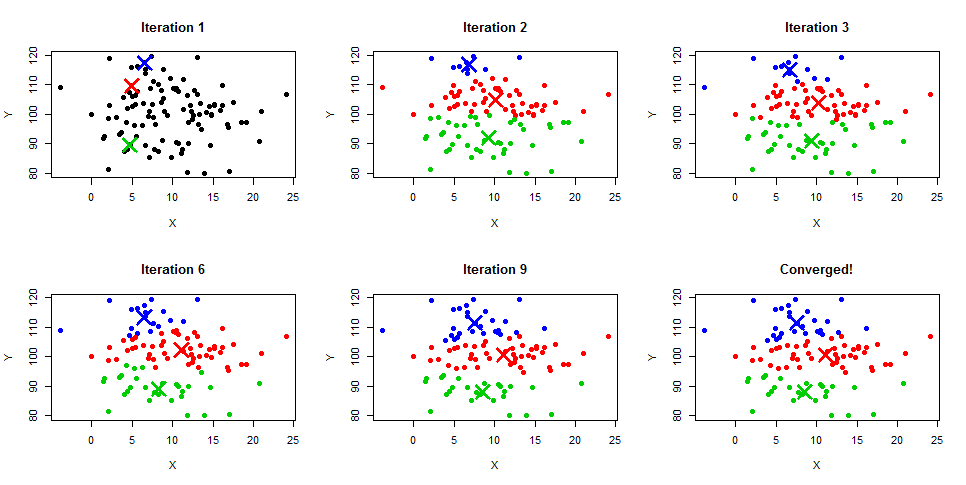
\includegraphics[width = 0.5\textwidth]{img/cluster/kmeans.png}
      \caption{Esempio di funzionamento dell'algoritmo $k-$means.}
      \label{img:k-means}
\end{figure}
Questo algoritmo è molto semplice da implementare e richiede un tempo di calcolo
pari a: $\mathcal{O}(t \cdot k \cdot n)$ con:
\begin{itemize}
      \item $n$ cardinalità dell'insieme dei dati.
      \item $k$ numero di cluster.
      \item $t$ numero di iterazioni del ciclo (avendo quindi $kt << n$)
\end{itemize}
\textbf{k-means} ha diversi problemi:
\begin{itemize}
      \item Ha una sensibilità rispetto alla scelta dei centroidi iniziali,
            sperimentalmente si è dimostrato che brutti valori iniziali
            invalidano l'intero processo.
      \item Non si può predire il numero di cluster non conoscendo a priori i
            dati, in aggiunta, non esiste un $k$ ottimale e non ci sono proprietà
            che ce lo possano suggerire. Si possono però usare delle
            approssimazioni studiando gli iperparametri. Non sapendo a priori il
            numero di $k$ posso ottenere scarsi risultati magari non avendo
            abbastanza centroidi. Adattarsi ad un numero “errato” di centroidi
            può portare a risultati “sporchi”.
      \item L'algoritmo è sensibile rispetto alle dimensioni geometriche che
            hanno le istanze nello spazio, infatti, lavorando sui centroidi
            potrebbe classificare in modo errato questo dettaglio, non
            distinguendo i corretti insiemi di punti.
      \item L'algoritmo è sensibile anche alla densità degli esempi, infatti se
            non avessimo $k$ sufficientemente grande allora si potrebbe arrivare
            a classificazioni errate.
\end{itemize}
In ogni caso, questo algoritmo mappa sensatamente i vari elementi in base alle
loro caratteristiche e quindi è un approccio parecchio usato, essendo generalmente
efficacie. Per risolvere i problemi introdotti precedentemente, si può provare
ad aumentare il numero di cluster, unendo poi, in un secondo passaggio, i vari
cluster secondo certi criteri, magari avendo una netta separazione lineare tra
cluster. Così si possono risolvere i problemi legati alla distribuzione geometrica
degli esempi, però rimane sempre il problema dell'identificare le posizioni di
inizializzazione dei centroidi migliori.
\section{Silhouette}
Per misurare le prestazioni di clustering bisogna capire come classificare i
risultati. Si usa la misura di \textbf{silhouette} per capire se un clustering è
migliore di un altro. Tale misura si basa sempre sul concetto di distanza.

Fissando una misura di distanza tra istanze $i, j$ ($d(i, j)$), definiremo:
\begin{enumerate}
      \item Distanza media \textbf{intra-cluster}, ovvero simiglianza tra
            elementi dello stesso cluster. Per ogni elemento $i$ di un cluster
            $C_I$, si calcola:
            \begin{equation}
                  a(i) = \frac{1}{|C_I| - 1} \sum_{j \in C_I, j \neq i} d(i, j)
            \end{equation}
            si divide per $|C_I| - 1 $ perché non si considera la distanza tra
            un elemento e se stesso.
      \item Distanza media \textbf{inter-cluster}, ovvero simiglianza tra un
            elemento di un cluster rispetto a tutti gli elementi tra gli altri
            cluster.  Per ogni elemento $i$ di un cluster $C_I$, si calcola:
            \begin{equation}
                  b(i) = \min_{K \neq I} \frac{1}{|C_K|} \sum_{j \in C_K} d(i, j)
            \end{equation}
            si divide per $|C_K|$ perché si considera la distanza tra un elemento
            e tutti gli elementi di un altro cluster.

            Si prende il minimo per confrontarlo con il cluster più vicino, anche
            detto \textbf{neighbor cluster}.
\end{enumerate}
Successivamente, si utilizzano le distanze precedenti per calcolare la silhouette 
per il punto $i$ nel seguente modo:
\begin{equation}
      s(i) = \frac{b(i) - a(i)}{\max\{a(i), b(i)\}}
\end{equation}
La qualità viene quindi visualizzata da un diagramma (come quelli riportati in
figura \ref{fig:silhouette}) che studia la silhouette al variare di $k$ per ogni
valore di ogni attributo (mettendo per ogni attributo in alto i valori più
studiabili).
\begin{figure}
      \centering
      \begin{subfigure}[b]{0.6\textwidth}
            \centering
            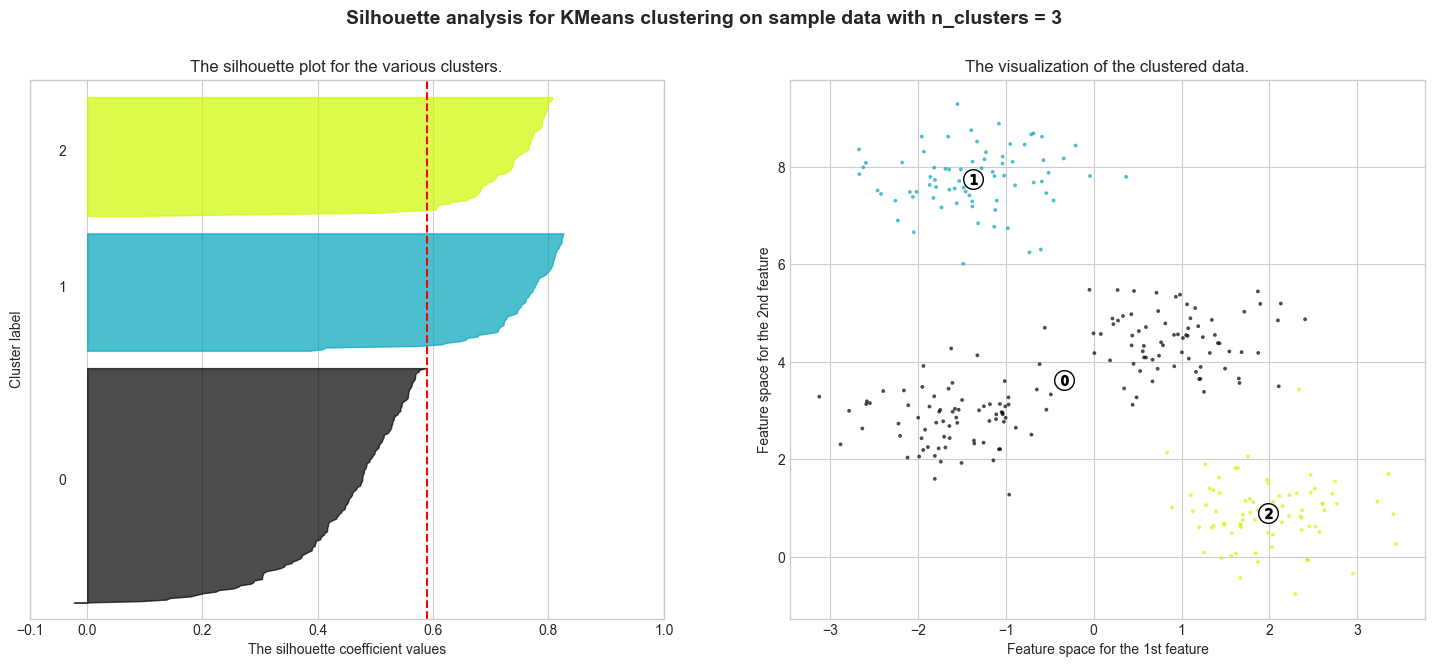
\includegraphics[width=\textwidth]{img/cluster/silhouette1.png}
            \caption{}
            \label{fig:silhouette1}
      \end{subfigure}
      \hfill
      \begin{subfigure}[b]{0.6\textwidth}
            \centering
            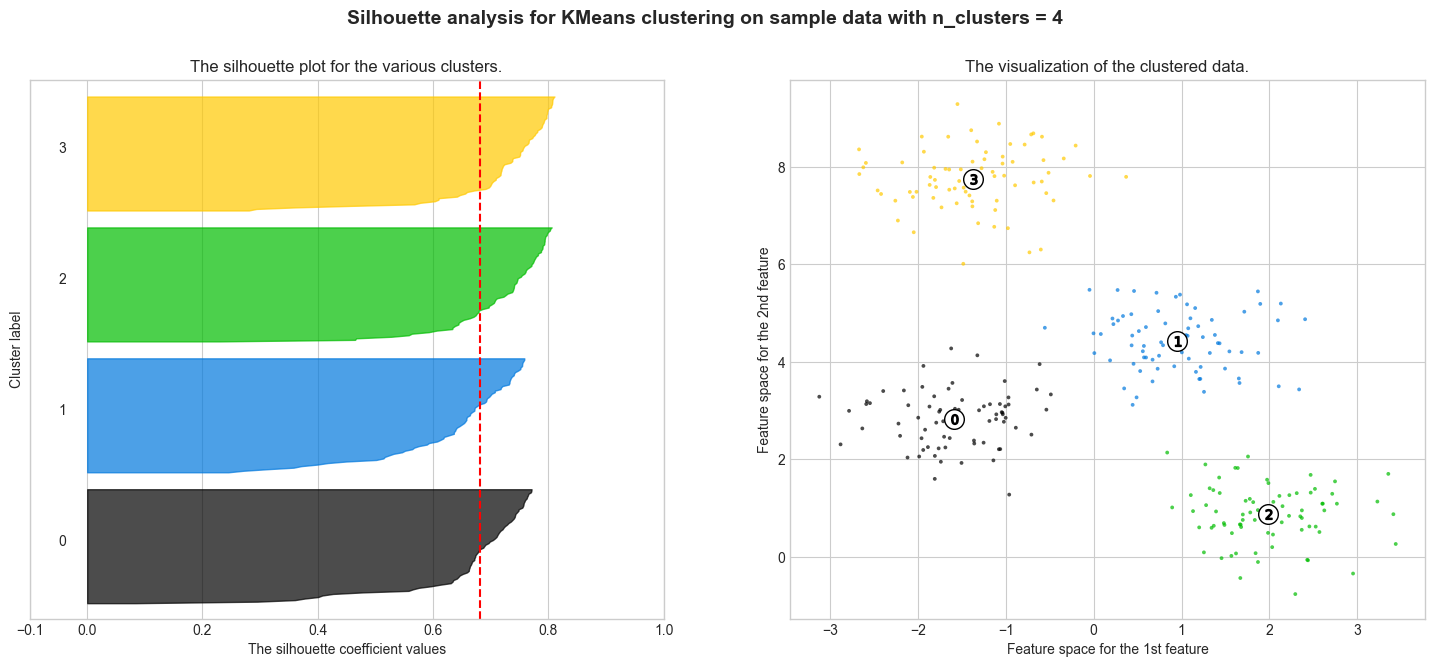
\includegraphics[width=\textwidth]{img/cluster/silhouette2.png}
            \caption{}
            \label{fig:silhouette2}
      \end{subfigure}
      \caption{Esempio di diagramma di silhouette.}
      \label{fig:silhouette}
\end{figure}
La media $s(i)$ su tutti i punti di un cluster è una misura di quanto siano
strettamente raggruppati tutti i punti del cluster. Pertanto, la media $s(i)$ su
tutti i dati dell'intero set di dati è una misura di quanto adeguatamente i dati
sono stati raggruppati. Se ci sono troppi o troppo pochi cluster, come può
accadere quando una scelta sbagliata di $k$ viene utilizzata nell'algoritmo di
clustering, alcuni dei cluster mostreranno tipicamente linee molto più strette
rispetto al resto nel diagramma di silhouette. Quindi, grafici e media di
silhouette possono essere utilizzati per determinare il numero “naturale” di
cluster all'interno di un set di dati.

Il valore della silhouette può variare da $-1$ a $1$, dove un valore alto indica
che gli oggetti sono ben raggruppati nel cluster e lontani dai cluster vicini.
Se molti punti hanno un valore alto, allora la configurazione del cluster è
appropriata. Se molti punti hanno un valore basso o negativo, allora la
configurazione del cluster può avere troppi o troppo pochi cluster.
Ad esempio:
\begin{itemize}
      \item Un valore medio della silhouette maggiore di $0,7$ è considerato un
            raggruppamento solido.
      \item Un valore medio della silhouette inferiore a $0,2$ indica che i
            dati potrebbero essere stati raggruppati in cluster errati.
\end{itemize}
La silhouette è utile quando i cluster hanno forme arbitrarie e potrebbe avere
problemi se i cluster hanno forme irregolari. Inoltre, posso usare una qualunque
misura di distanza.